\subsection{Définition}
Un compteur intelligent est un compteur électronique qui mesure la quantité d'énergie consommée sur une période de temps définie. Il communique et transmet également des données de consommation, comme vos index, et peut recevoir des informations ou des ordres à votre demande. Il offre ainsi de nouveaux services sans rendez-vous et sans dérangement pour vous. 

Tous les compteurs intelligents affichent en permanence 4 index, peu importe que vous ayez une production d'énergie (par exemple, des panneaux photovoltaïques) et peu importe votre choix tarifaire (simple tarif, bi-horaire,...)  : 

\begin{itemize}[label=\textbullet]
\item la consommation aux heures pleines 
\item la consommation aux heures creuses 
\item l'injection d'énergie aux heures pleines 
\item l'injection d'énergie aux heures creuses
\end{itemize}

\begin{figure}[h]
	\centering
    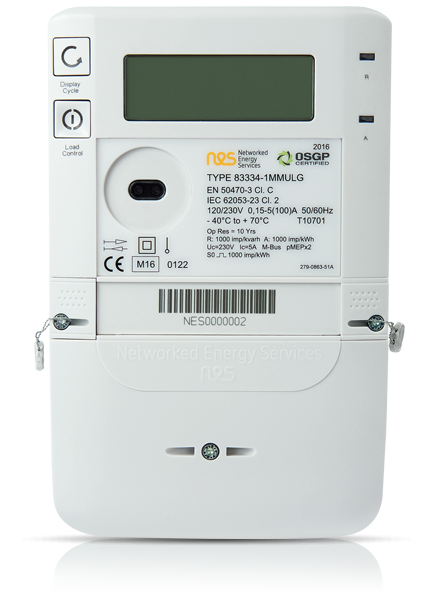
\includegraphics[scale=0.4]{img/part2/1.4}
    \caption{Exemple de compteur intelligent}
\end{figure}